%(Summary and Interpretation) 

The relative suppression of the $\PgU$ excited states has been measured, based on the first $150 \mu b^{-1}$ of the 2011 \PbPb dataset.
The observed results ($\chi_{2}\equiv 2S/1S=0.21 \pm 0.07 \pm 0.02$ and $\chi_{23}\equiv(2S+3S)/1S=0.15 \pm 0.05 \pm 0.02$) are considerably more precise than, and found compatible with, the published measurements based on the 2010 PbPb dataset. 
%
%Significance estimations , employing the generation of large pseudo-experiments, were performed based on the partial dataset used in the current version of this document and non-final systematic evaluation. 
%An observation of the double ratio $\chi_{23}$ below 0.5 will yield a significance larger than $3\,\sigma$.  
%A significance in excess of $5 \sigma$ is attained. 
Profile likelihood based estimations show the significance of the relative excited-to-ground state suppression is larger than $5\,\sigma$.
The larger luminosity of the \PbPb dataset further allows to carry out the measurement in ranges of the dimuon kinematics and the centrality of the collision. 
No definitive trend is identified with the current precision. 
A clear dependence on the collision centrality is observed for the nuclear modification factors for the individual $\PgUa$ and $\PgUb$ states. 
The $\PgUc$ state is not shown prominently in the \PbPb data. 
An upper limit on the 3S/1S double ratio is set at 95\% C.L..
 
\vfill

\begin{figure}[hbtp]
  \begin{center}
    \subfigure[2010]{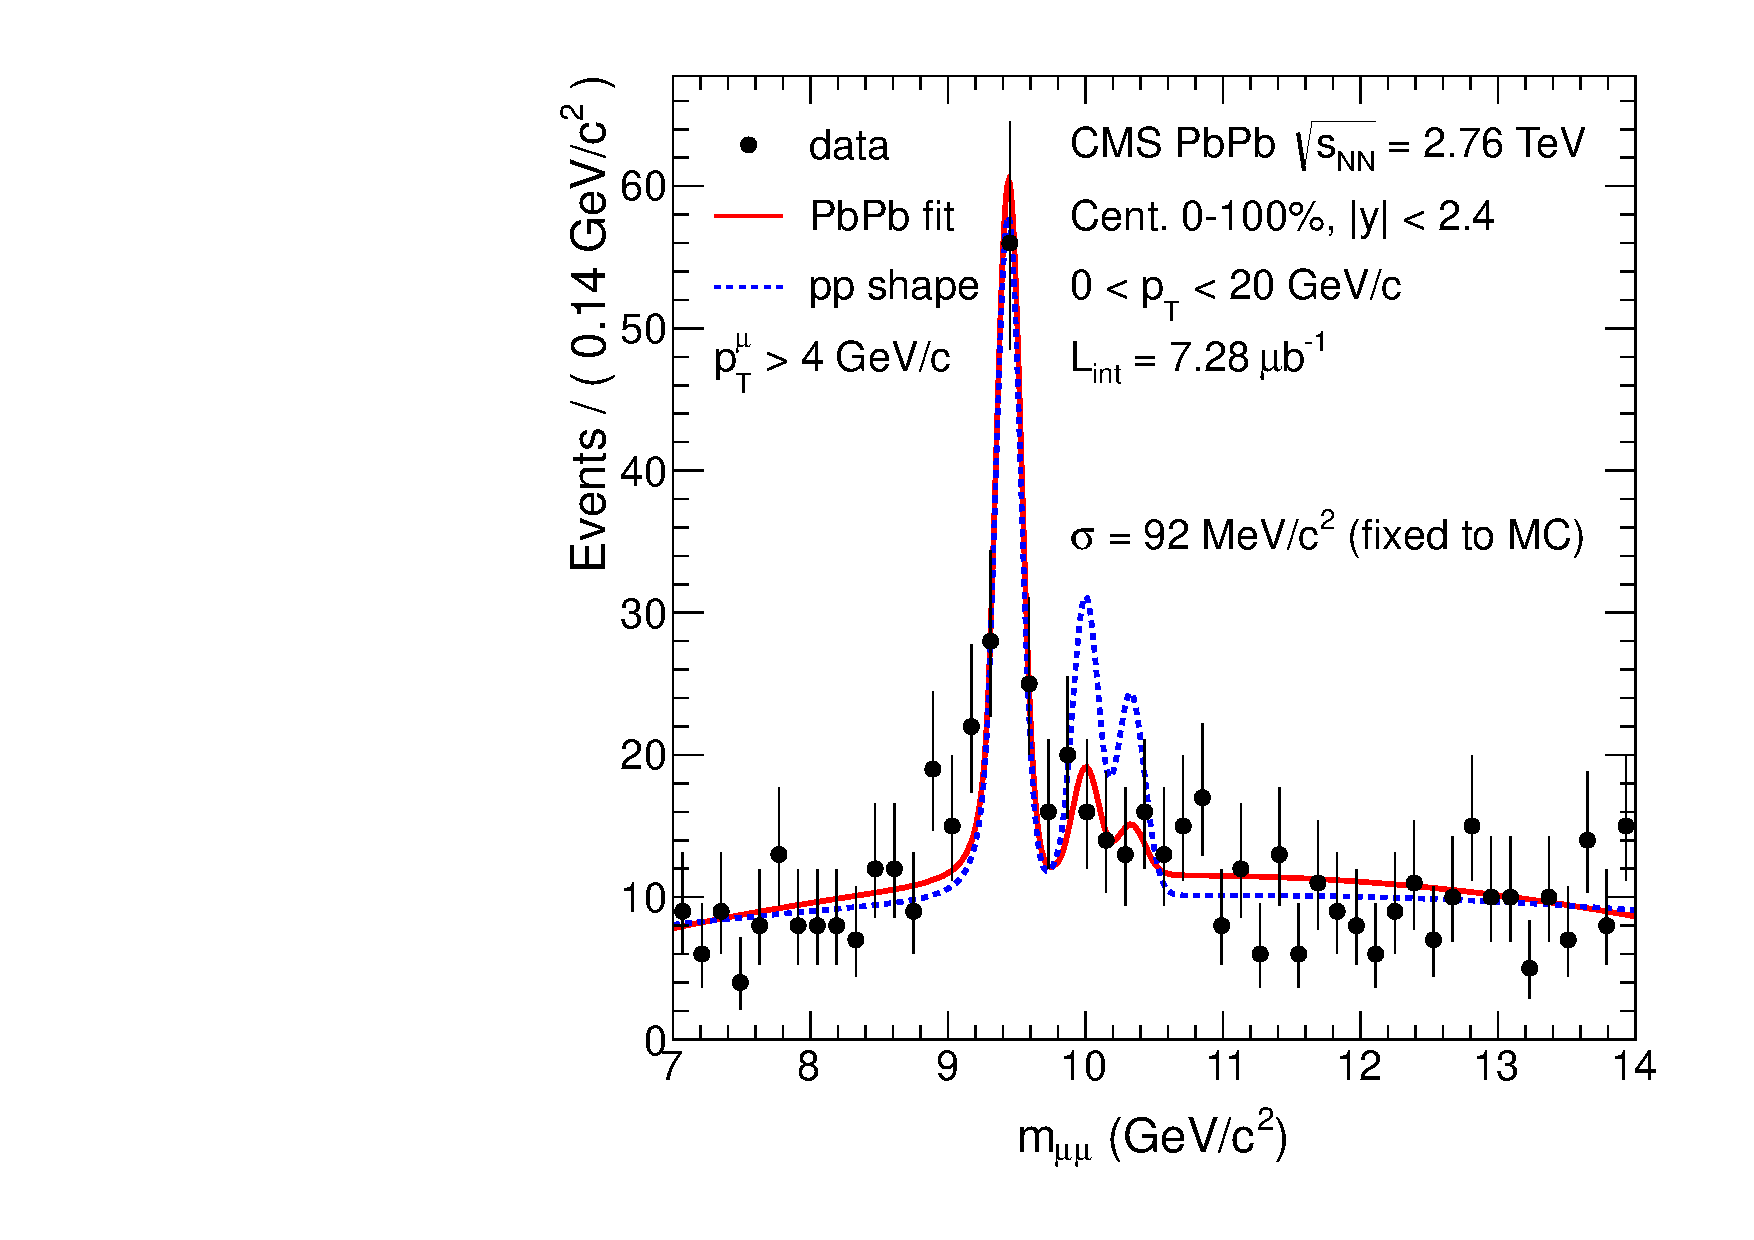
\includegraphics[angle=0,width=0.5\textwidth]{figures/fulldataset/overlay1_masspeak_Hi2010}}
    \subfigure[2011]{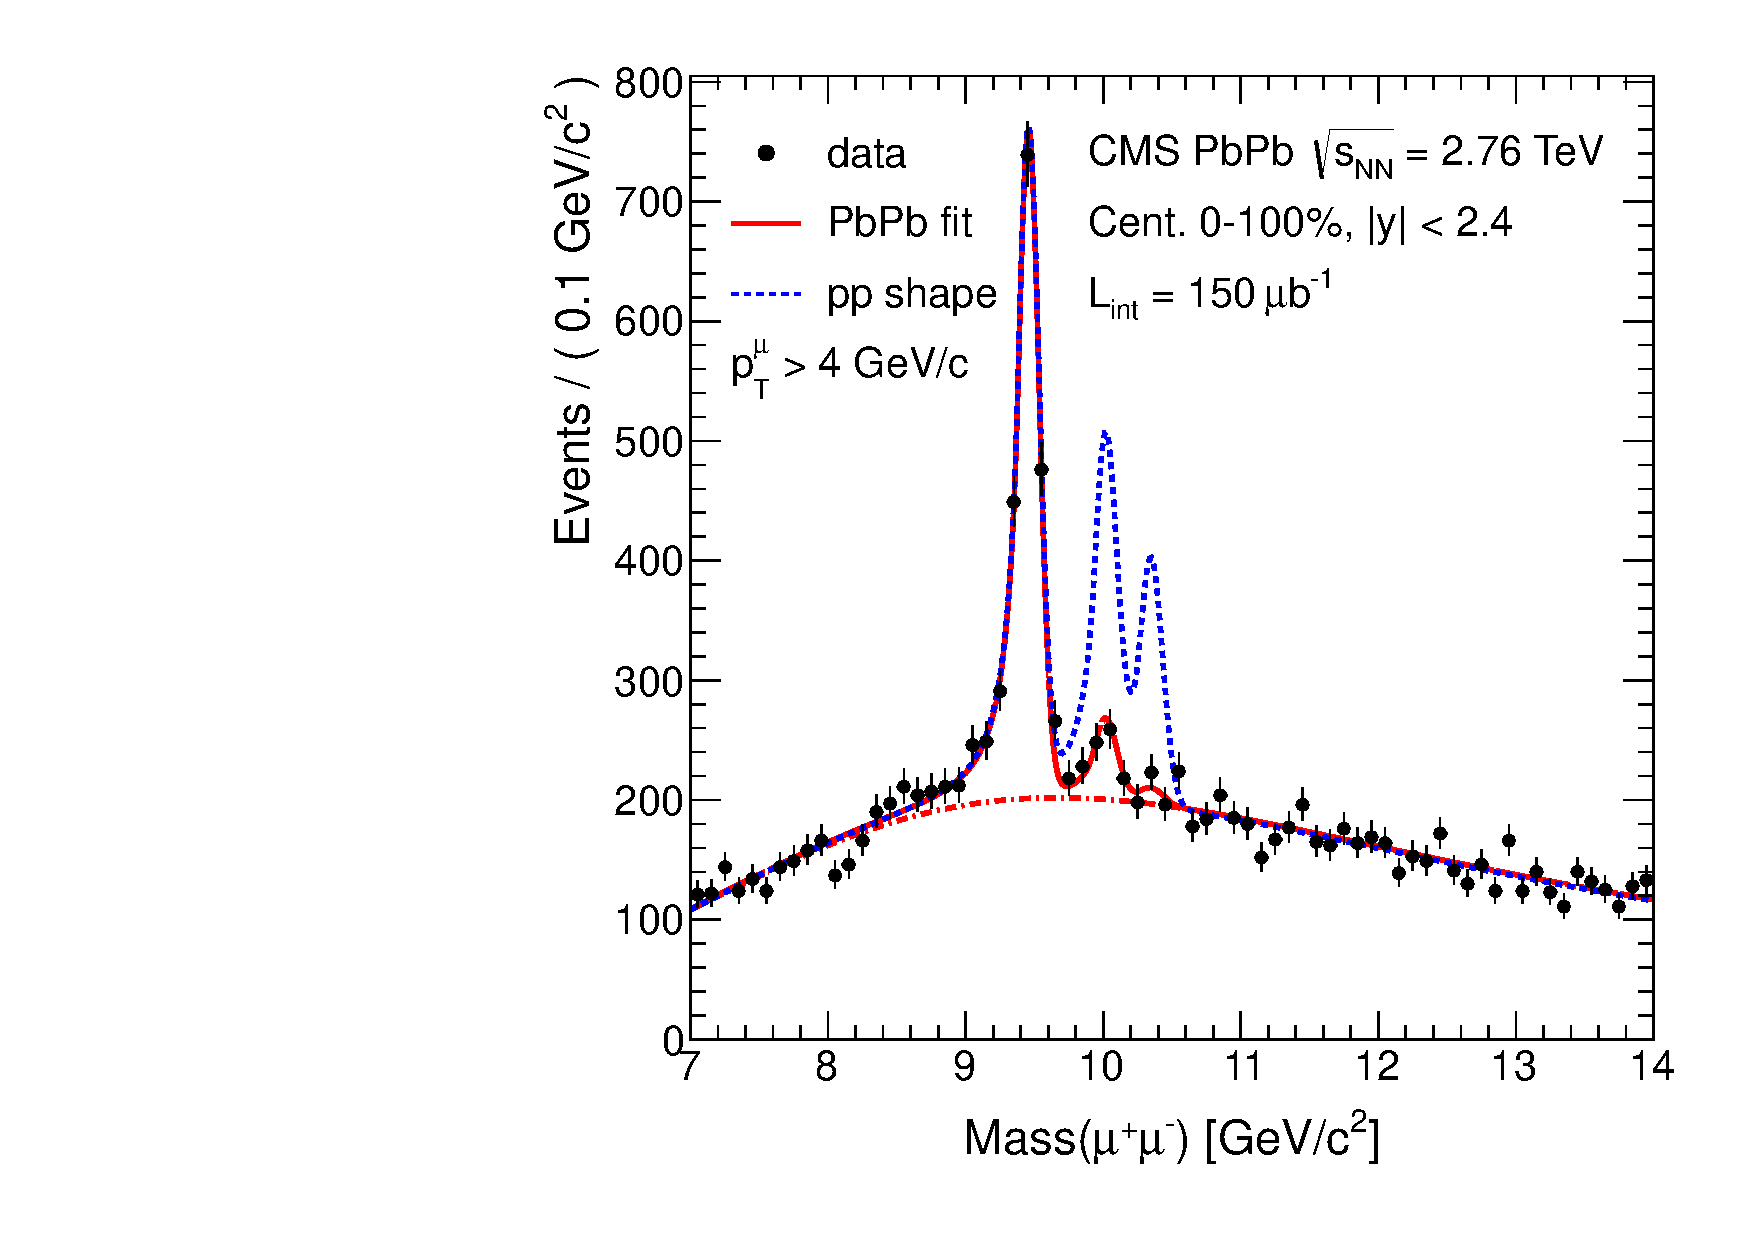
\includegraphics[angle=0,width=0.5\textwidth]{figures/fulldataset/overlay2_masspeak_Hi}}
    \caption{Illustration of the excited to ground states relative \PgU\ suppression in \PbPb compared to \pp, and comparison of the effect observed using the 2010 \emph{(left)} and 2011 \emph{(right)} \PbPb datasets. The fit to the \PbPb data, shown  by the continuous line, is overlaid with the result of the \pp fit, represented by the dashed line (shown on top of a common \PbPb background shape, for comparison).  For a better comparison, the background shape, background yield, mass peak width, mass peak tail shape and the \PgUa yields in the red line are fixed to the PbPb fit, while the \PgUb/\PgUa and \PgUc/\PgUa ratios are fixed to the pp fit values.  These plots are provided for illustration, and do not reflect the analysis details.}
    \label{fig:pr-overlay}
  \end{center}
\end{figure}

\begin{figure}[hbtp]
  \begin{center}
    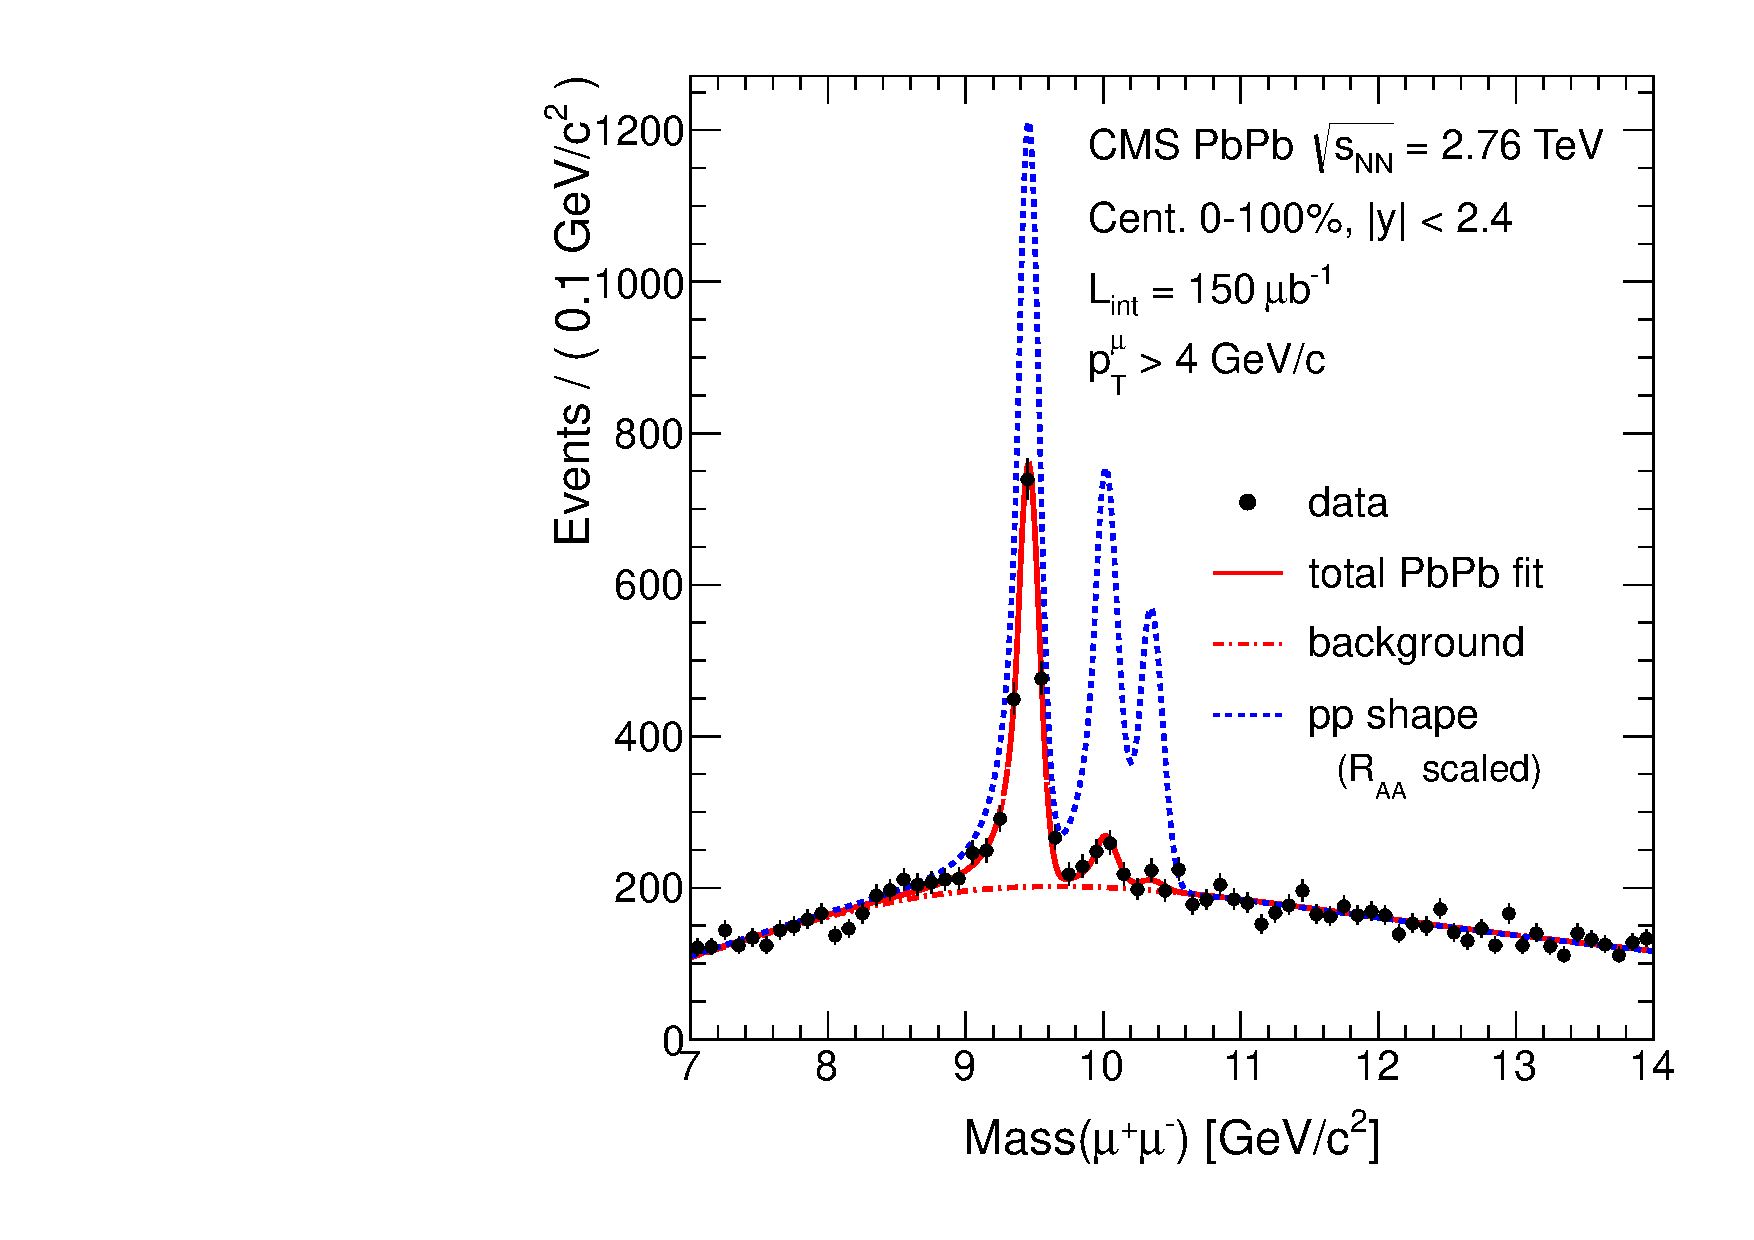
\includegraphics[angle=0,width=0.5\textwidth]{figures/fulldataset/overlay5_masspeak_Hi.pdf}
    \caption{Dimuon invariant-mass distribution from the \PbPb data, with the fit results shown as the solid (data + background) and dot-dashed (background-only) lines. The dashed curve illustrates the corresponding signals in \pp data, scaled by the \raa values. The same reconstruction algorithm and analysis criteria are applied to the \PbPb and \pp datasets, including a transverse momentum requirement on single muons of $\pt > 4 \GeVc$. }
    \label{fig:PRplot_raa}
  \end{center}
\end{figure}



\vfill


